\documentclass[tikz,border=6pt]{standalone}
\usepackage{amsmath}
\usetikzlibrary{arrows.meta,positioning,calc}
\begin{document}
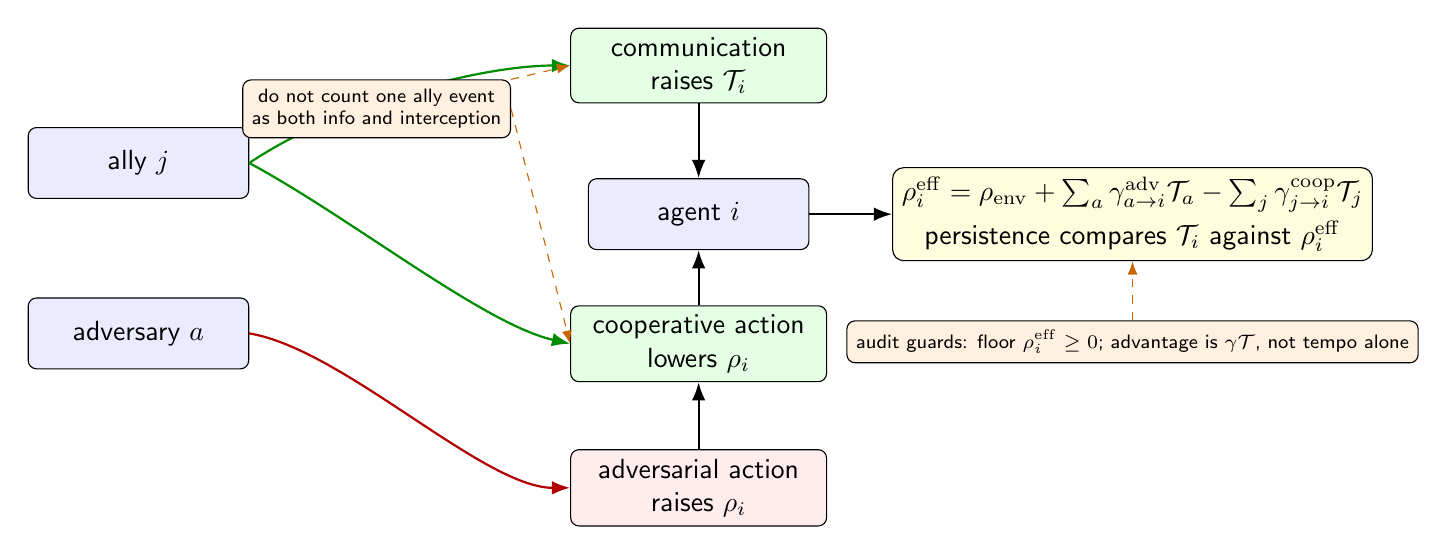
\begin{tikzpicture}[
  font=\sffamily,
  >=Latex,
  agent/.style={draw, rounded corners=3pt, fill=blue!8, align=center, minimum width=2.8cm, minimum height=0.9cm},
  lever/.style={draw, rounded corners=3pt, fill=green!10, align=center, minimum width=3.25cm, minimum height=0.85cm},
  disturb/.style={draw, rounded corners=3pt, fill=red!7, align=center, minimum width=3.25cm, minimum height=0.85cm},
  formula/.style={draw, rounded corners=4pt, fill=yellow!13, align=center, minimum width=5.3cm, minimum height=1.1cm},
  warn/.style={draw, rounded corners=3pt, fill=orange!12, align=center, font=\sffamily\scriptsize}
]

\node[agent] (ally) {ally $j$};
\node[agent, below=1.25cm of ally] (adv) {adversary $a$};
\node[agent, right=4.3cm of ally, yshift=-0.65cm] (target) {agent $i$};

\node[lever, above=0.95cm of target] (comm) {communication\\raises $\mathcal T_i$};
\node[lever, below=0.7cm of target] (coop) {cooperative action\\lowers $\rho_i$};
\node[disturb, below=0.85cm of coop] (attack) {adversarial action\\raises $\rho_i$};

\draw[->, thick, green!55!black] (ally.east) .. controls +(1.2,0.8) and +(-1.1,0) .. (comm.west);
\draw[->, thick, green!55!black] (ally.east) .. controls +(1.3,-0.7) and +(-1.1,0.25) .. (coop.west);
\draw[->, thick, red!70!black] (adv.east) .. controls +(1.2,-0.2) and +(-1.1,0) .. (attack.west);

\draw[->, thick] (comm.south) -- (target.north);
\draw[->, thick] (coop.north) -- (target.south);
\draw[->, thick] (attack.north) -- (coop.south);

\node[formula, right=1.05cm of target] (ledger)
  {$\rho_i^{\mathrm{eff}}=\rho_{\rm env}
    +\sum_a \gamma^{\rm adv}_{a\to i}\mathcal T_a
    -\sum_j \gamma^{\rm coop}_{j\to i}\mathcal T_j$\\[2pt]
   persistence compares $\mathcal T_i$ against $\rho_i^{\mathrm{eff}}$};

\draw[->, thick] (target.east) -- (ledger.west);

\node[warn, below=0.75cm of ledger, minimum width=5.3cm] (floor)
  {audit guards: floor $\rho_i^{\rm eff}\ge 0$; advantage is $\gamma\mathcal T$, not tempo alone};
\draw[->, dashed, orange!80!black] (floor.north) -- (ledger.south);

\node[warn, left=0.75cm of comm, yshift=-0.55cm, minimum width=2.9cm] (double)
  {do not count one ally event\\as both info and interception};
\draw[->, dashed, orange!80!black] (double.east) -- (coop.west);
\draw[->, dashed, orange!80!black] (double.north east) -- (comm.west);

\end{tikzpicture}
\end{document}
